\documentclass[main.tex]{subfiles}
\begin{document}
	
	% TODO: extensions are module specific, various extensions, coprehensive understanding, purpose of following sections 
	% TODO: introductory paragraph
	
	Different compilers can support different language extensions. Throughout the rest of this chapter, we will discuss the extensions provided by the Glasgow Haskell Compiler, the most widely used Haskell compiler. GHC implements a daunting number of 110 extensions. It would be difficult to deal with every single language extension, so we will consider only those that are used in more than one thousand modules throughout the Hackage database \cite{hackage-bib}, and those that are closely related to them. We found over 30 extensions satisfying this criteria. Together they cover more than 90\% of the total occurrences of all extensions. We categorized them based on their functionalities, and measured their relative usage statistics. These statistics can be seen in Diagram~\ref{fig:rel-ext-piechart}.
	
	\begin{figure}[h]
		\renewcommand{\figurename}{Diagram}
		\hspace{-1cm}
		\centering
		\caption{Relative extension usage statistics}
		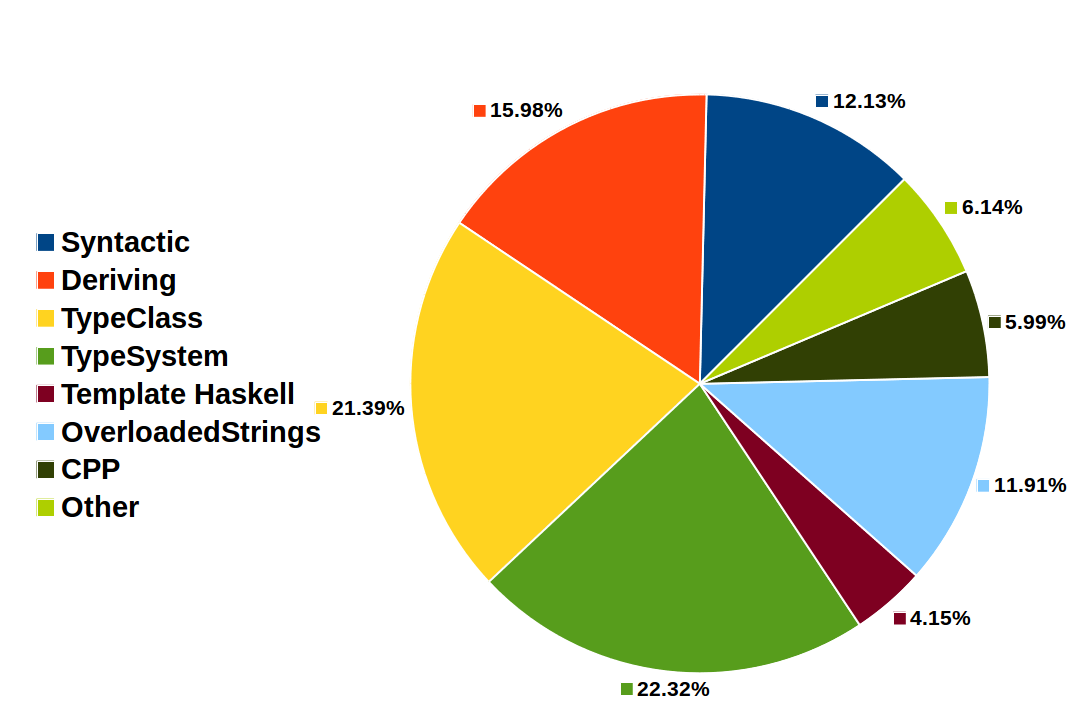
\includegraphics[scale=0.5]{extension_categories_pie}
		\label{fig:rel-ext-piechart}
	\end{figure}
		
	\section{Implication relations}
	
	By defining such a wide range of many different extensions, some relations naturally form between certain extensions. The language extensions supported by GHC have so-called \emph{implication relations} defined over them. Extension \textbf{A} \emph{implies} extension \textbf{B} if and only if turning on \textbf{A} requires turning on \textbf{B}. These implication relations are implicit, which means turning on an extension implicitly turns on all corresponding implied extensions. For instance, if we use \ext{GADTs} in our module, then (besides others extensions) \ext{GADTSyntax} is automatically turned on for us, we do not have to turn it on manually. It is also worth mentioning, that the implication relation is transitive.
	
	The complete network of implication relations among the extensions supported by GHC can be represented by a group of directed acyclic graphs, as shown in Figures~(\ref{fig:explicit-namespaces-dag})--(\ref{fig:others-dag}). In these graphs only the immediate implications are illustrated, transitive ones are not.
	
	The implication relations play a crucial role from the perspective of extension elimination. In order to remove a certain extension from a module, we must be able to determine if the extension is necessary. We can achieve this by analyzing the syntax tree of the module, and finding all the language elements requiring the given extension. If we did not find any language elements, we can safely remove the extension.	We define so-called \emph{checkers} for each individual extension, which are responsible for finding the language elements requiring the corresponding extension. If extension \textbf{A} implies extensions \textbf{B} and \textbf{C}, after eliminating \textbf{A}, we must explicitly turn on \textbf{B} and \textbf{C}, because the module might still use the functionalities provided by the latter two. If we want to completely remove \textbf{A}, we must define checkers for the other two extensions as well. Unfortunately, in some cases this is not possible.
	
	%\subfile{extension_relations_forest}
	
	
\end{document}